%!TEX root = skripsi.tex
%-----------------------------------------------------------------------------%
\chapter{\babTiga}\label{bab:tiga}
%-----------------------------------------------------------------------------%
%-----------------------------------------------------------------------------%
% Ide, model matematik, rumus, fitur, jangan m=ngomongin teknologi (java, keras, dll), word2vec boleh %
In this chapter, we describe the methodology used in this research. It consists of data gathering, data pre-processing, data annotation, experiment, and evaluation. Before we describe each part in details, we explain the big picture of the methodology in a form of pipeline.

\section{Pipeline}
The goal of this research is to build a model that predicts the semantic roles of each Indonesian sentence. In other languages such as English, there are already semantic role corpus from which the SRL system is built. Unfortunately, that is not the case for Indonesian, since there is no annotated corpus available yet. We therefore create our own with the annotation guideline crafted for Indonesian conversational language. In this research, we focus on building SRL system for the conversational Indonesian language.

We view SRL as a sequence labeling problem. Suppose that we have an input of \textit{n} words $w = (w_{1}, w_{2}, ..., w_{n})$, the goal is to find the best label sequence $y = (y_{1}, y_{2}, ..., y_{n})$, with $y_{i}$ representing the semantic roles. The probabilities of the label in each time step $i$ is described as follows.
\begin{equation}
P(y_{i}|w_{i-l}, ..., w_{i+l},y_{i-l}, ..., y_{i+l})
\end{equation}

whereby \textit{l} is a small number. In this section, we explain our research methodology including the data annotation, features used, and the proposed model architecture. 

This research uses the data from one of Kata.ai's chat bots. Firstly, the data is pre-processed before going into the next steps. After that, the data is then annotated with semantic roles based on the annotation guideline proposed by us for Indonesian conversational language. The annotated data is then divided into training, development, and testing sets with the ratio of 80:20:20, respectively.

There are 2 main scenarios for the experiment. The first scenario aims for finding the best set of features that output the best performance. The goal of the second scenario is to find which deep learning model architecture has the best result. In the first scenario, we have two features, which are word embedding and POS Tag. In the second scenario, we compare four model architectures, namely vanilla Long Short-Term Memories (LSTM), Bi-Directional LSTM (BLSTM), CNN-BLSTM, and Context-Aware BLSTM (CA-BLSTM).

Every experiment is evaluated based on precision, recall, and F-measure of each semantic roles. The evaluation approach used is partial match based on Seki et al. (20xx). We then analyze and explain the results of each experiment scenario.

\section{Data Gathering}
In this research we use real-world data from one of Kata.ai chat bots. We firstly retrieved data consisting of 40.000 instances of text chats. We then manually deleted junk chats which contain, for example, only laugh or greeting. After that, we run a script to delete duplicate chats. The deletion process outputs a clean data with 30.000 instances in total. Finally, we randomly selected 9.000 out of 30.000 instances as the data to be annotated. This data set will be the one which is trained and tested to build the SRL system.

It is worth to note that conversational language has unique characteristics. First, they use slangs and abbreviations. For example, one might use \textit{"u"} instead of \textit{"you"} in \textit{"I brought u a present"}. The grammars are often unstructured and thus, one cannot rely on syntactic parsers to build SRL system for conversational language. The sentences are also filled with interjections such as \textit{"haha"} and \textit{"lol"}. Lastly, since conversational sentences are really short, averaging around 5-7 words per sentence, it sometimes contains incomplete information. These are the interesting challenges the SRL system should learn and tackle.

\section{Data Pre-Processing}
After the data has been gathered, the next step is to pre-process the data so that it could be fed into the machine learning model later. In this step, each sentence is going through a process called tokenization. Tokenization splits sentence into its individual words. Traditionally, one can split sentence by \textit{space}, however, it does not work for sentences in conversational language since number or symbol are often concatenated with words, such as "makan2". It thus needs further tokenization technique, that is, splitting alphabet with number and symbol tokens. This way, "makan2" will be tokenized as "makan 2". In addition to tokenization by \textit{space}, the rules are listed as follows:

\begin{enumerate}
	\item <alphabet><numeric> to be <alphabet><space><numeric>
	\item <numeric><alphabet> to be <numeric><space><alphabet>
	\item <alphabet><symbol> to be <alphabet><space><symbol>
	\item <symbol><alphabet> to be <symbol><space> <alphabet>
\end{enumerate}

Figure~\ref{fig:tokenization} illustrates a few examples of sentence tokenization.
\begin{figure}
	\centering
	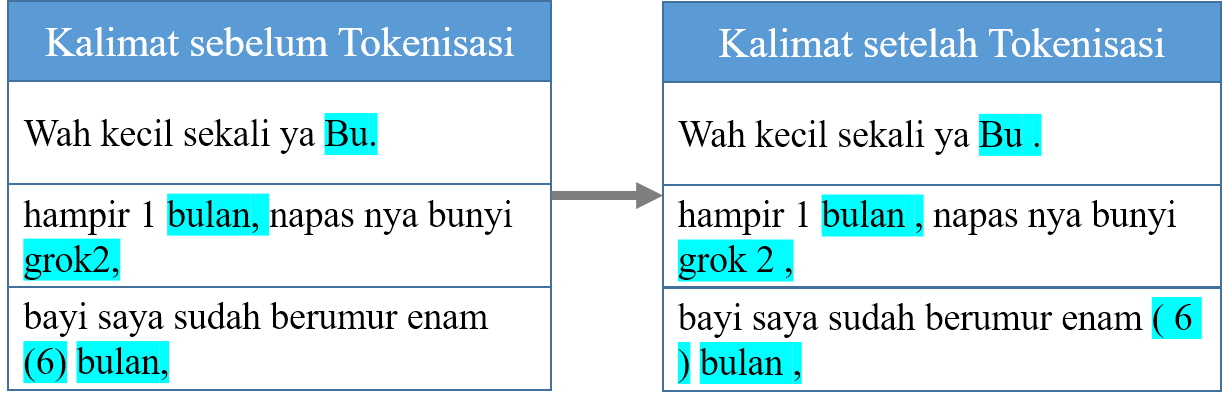
\includegraphics[width=\linewidth]{images/tokenisasi}
	\caption{Sentence Tokenization Illustration}
	\label{fig:tokenization}
\end{figure}

\section{Data Annotation}
In this work, we create a new set of semantic roles mainly crafted for informal conversational language. The summary of semantic roles proposed with its examples are presented in Table~\ref{tab:semantic_roles}.

\begin{table}
	\centering
	\caption{Set of Semantic Roles for Conversational Language}
	\label{tab:semantic_roles}
	\begin{tabular}{|l|l|}
		\hline
		\multicolumn{1}{|c|}{Semantic Roles} & \multicolumn{1}{c|}{\textit{Example}} \\
		\hline
		\textsc{Agent}		& \underline{Aku} beliin kamu kado\\
		\textsc{Patient}		& Aku beliin kamu \underline{kado}\\
		\textsc{Beneficiary}	& Aku beliin \underline{kamu} kado\\
		\textsc{Greet} 				& Hai \underline{Budi}! Aku beliin kamu kado\\
		\textsc{Modal} 				& Aku \underline{bisa} makan di rumah besok\\
		\textsc{Location} 			& Aku bisa makan di \underline{rumah} besok\\
		\textsc{Time} 				& Aku bisa makan di rumah \underline{besok} \\
		\hline
	\end{tabular}
\end{table}

These semantic roles are mainly inspired by the work of \cite{saeed19972003}, except that \textsc{Agent} and \textsc{Patient} refer to \textsc{Proto-Agent} and \textsc{Proto-Patient} as explained by \cite{dowty1991thematic}. The main difference of this set of semantic roles compared to the previous ones is \textsc{Greet}.

The center of all semantic roles is the \predicate. As in English, \predicate in Indonesian is usually in a form of \textit{verb}, as illustrated by the examples below:
\begin{description}
	\item[$\bullet$] "Kemarin aku \underline{makan} di rumah"
	\item[$\bullet$] "Aku \underline{ada} ujian nih hari Senin"
\end{description}

In Indonesian, however, predicate can also be an adjective. Some examples are presented as follows:
\begin{description}
	\item[$\bullet$] "Kamu \underline{cantik} deh"
	\item[$\bullet$] "Aku lagi \underline{sedih} nih"
\end{description}

In this section, we briefly explain each semantic roles with their respective examples.
\begin{enumerate}
	\item \agent\\
	An entity is called as \agent~ if one of this following properties is fulfilled:
	\begin{description}
		\item Volitional involvement in event or state
		\item Sentience (and/or perception)
		\item Causing an event or change of state in another participant
		\item Movement (relative to position of another participant) (exists independently of event named)
	\end{description}
	
	The examples of \agent~ in a sentence are given as follows:
	\begin{description}
		\item[$\bullet$] "\underline{Aku} makan ayam dulu ya"
		\item[$\bullet$] "\underline{Kamu} gak tidur?"
		\item[$\bullet$] "\underline{Kamu} mau beliin aku pulsa?"
	\end{description}
	
	\item \patient\\
	An entity is called as \patient~ if one of this following properties is fulfilled:
	\begin{description}
		\item Volitional involvement in event or state
		\item Sentience (and/or perception)
		\item Causing an event or change of state in another participant
		\item Movement (relative to position of another participant) (exists independently of event named)
	\end{description}
	
	The examples of \patient~ in a sentence are given as follows:
	\begin{description}
		\item[$\bullet$] "Aku makan \underline{ayam} dulu ya"
		\item[$\bullet$] "Kamu mau beliin aku \underline{pulsa}?"
		\item[$\bullet$] "\underline{Aku} lagi sedih nih.."
	\end{description}

	\item \beneficiary\\
	\beneficiary~ is an entity which gets benefit of the predicate. It is usually in a form of indirect object. The examples of \beneficiary~ in a sentence are given as follows:
	\begin{description}
		\item[$\bullet$] "Kamu mau beliin \underline{aku} pulsa?"
		\item[$\bullet$] "Aku pengen ngobrol sama \underline{kamu}"
	\end{description}
	
	\item \greet\\
	\greet~ is the main difference of this set of semantic roles for conversational language. \greet~ refers to an animate object, usually a person, which is being greeted in a chat. In conversational language, one often calls the name of person it is talking to. This information is useful, for instance, we can derive that \textit{"you"} refers to \textit{"Budi"} in \textit{"Halo Budi! Aku beliin kamu kado loh"}. The examples of \greet~ in a sentence are given as follows:
	\begin{description}
		\item[$\bullet$] "Hai \underline{rizky}! kamu udah makan belum?"
		\item[$\bullet$] "aku ga bisa tidur nih \underline{Val}"
	\end{description}

	\item \modal\\
	\modal~ refers to \textit{modal verb} of a predicate. The word examples are \textit{"boleh, harus, pernah, sudah, udah, mesti, perlu, akan, lagi, bisa, mau, ingin, pengen, pingin"}. The examples of \modal~ in a sentence are given as follows:
	\begin{description}
		\item[$\bullet$] "Aku \underline{mau} makan dulu ya!"
		\item[$\bullet$] "Kamu \underline{udah} tidur belum?"
	\end{description}

	\item \location\\
	\location~ refers to the location of a predicate. The examples of \location~ in a sentence are given as follows:
	\begin{description}
		\item[$\bullet$] "Aku mau makan di \underline{rumah} ya!"
		\item[$\bullet$] "Kamu gak pergi ke \underline{sekolah}?"
	\end{description}

	\item \timesrl\\
	\timesrl~ refers to the time of a predicate. The examples of \timesrl~ in a sentence are given as follows:
	\begin{description}
		\item[$\bullet$] "\underline{Kemarin} aku makan di rumah"
		\item[$\bullet$] "Aku ada ujian nih \underline{hari Senin}"
	\end{description}
\end{enumerate}

Following Collobert et al., all the labels are tagged using BIO (Begin Inside Outside) tagging~\cite{collobert2011natural}. Suppose that a label \patient consists of more than one word, such as \textit{"ayam goreng"} in "Aku makan \textit{ayam goreng}", "ayam" and "goreng" are tagged as "B-Patient" and "I-Patient", respectively. If the label has only one word, than it is tagged as "B-Patient". Word that does not have any label is thus tagged as "O" which means "Others".

After the data has been labeled, the labels need to be encoded in a way the deep learning model understands. To do so, the labels are then transformed into \textit{one-hot-vector}. Each label is mapped into a unique one-hot-vector, hence the relation is 1-to-1.
\begin{table}
	\centering
	\caption{Set of Semantic Roles for Conversational Language}
	\label{tab:examplelabel}
	\begin{tabular}{|lcccc|}
		\hline
		\textbf{Sentence} 				& Aku & pengen & makan & ayam \\
		\hline
		\textbf{BIO-Label}				& B-AGEN & B-MD & B-PRED & B-PATIENT  \\
		\hline
		\textbf{One-Hot-Vector}		& [1, 0, 0, .., 0] & [0, 1, 0, .., 0] & [0, 0, 1, .., 0] & [0, .., 1, 0, 0] \\
		\hline
	\end{tabular}
\end{table}

Table~\ref{tab:examplelabel} shows an example of how sentence is labeled with the one-hot vectors representations of BIO format.

\section{Model Development}
In this section, the features and model architecture are described. We firstly describe word embedding and POS Tag as the feature candidates. Following after that, the four model architectures, one of which is the new architecture we propose, are explained.

\subsection{Feature Extraction}
In this step, we extract features from the data that has been annotated with semantic roles. We propose three features which will be combined later to find the best feature selection that outputs the best result. Those features are word embedding, POS-Tag, and neighboring word embeddings.

\subsubsection{Word Embedding}
% Apa itu word embedding
Word embedding represents word as a vector. Word embedding has proved to be one of the most contributing features by a lot of deep learning research, such as for SRL system proposed by \cite{zhou2015end} and \cite{collobert2011natural}. The interesting characteristic of word embedding is that similar words have proved to have similar vectors. This is very important when dealing with conversational language which has a lot of slang words. For instance, pronoun "Aku" will have similar vector with its slang form, "Gue". We believe that this feature will contribute greatly to the model performance. Therefore, we utilized our embedding as one of our feature candidates.

% Cara mendapat word embedding model
In order to utilize word embedding as our features, we conduct three steps which consist of: 1.) data gathering for building word embedding model, 2.) training the word embedding model, and 3.) converting words into vectors with the trained word embedding model.

\begin{enumerate}
	\item Data gathering for building word embedding modelPengumpulan data \textit{training} untuk \textit{word embedding}\\
	%Berikan penjelasan
	
	\item Training the word embedding model\\
	%Berikan penjelasan
	
	\item Converting words into vectors with the trained word embedding model\\
	%Berikan penjelasan
	
\end{enumerate}

Figure~\ref{fig:wordembedding} illustrates the afore-mentioned steps in order to get the vector representation of words with word embedding.

\begin{figure}
	\centering
	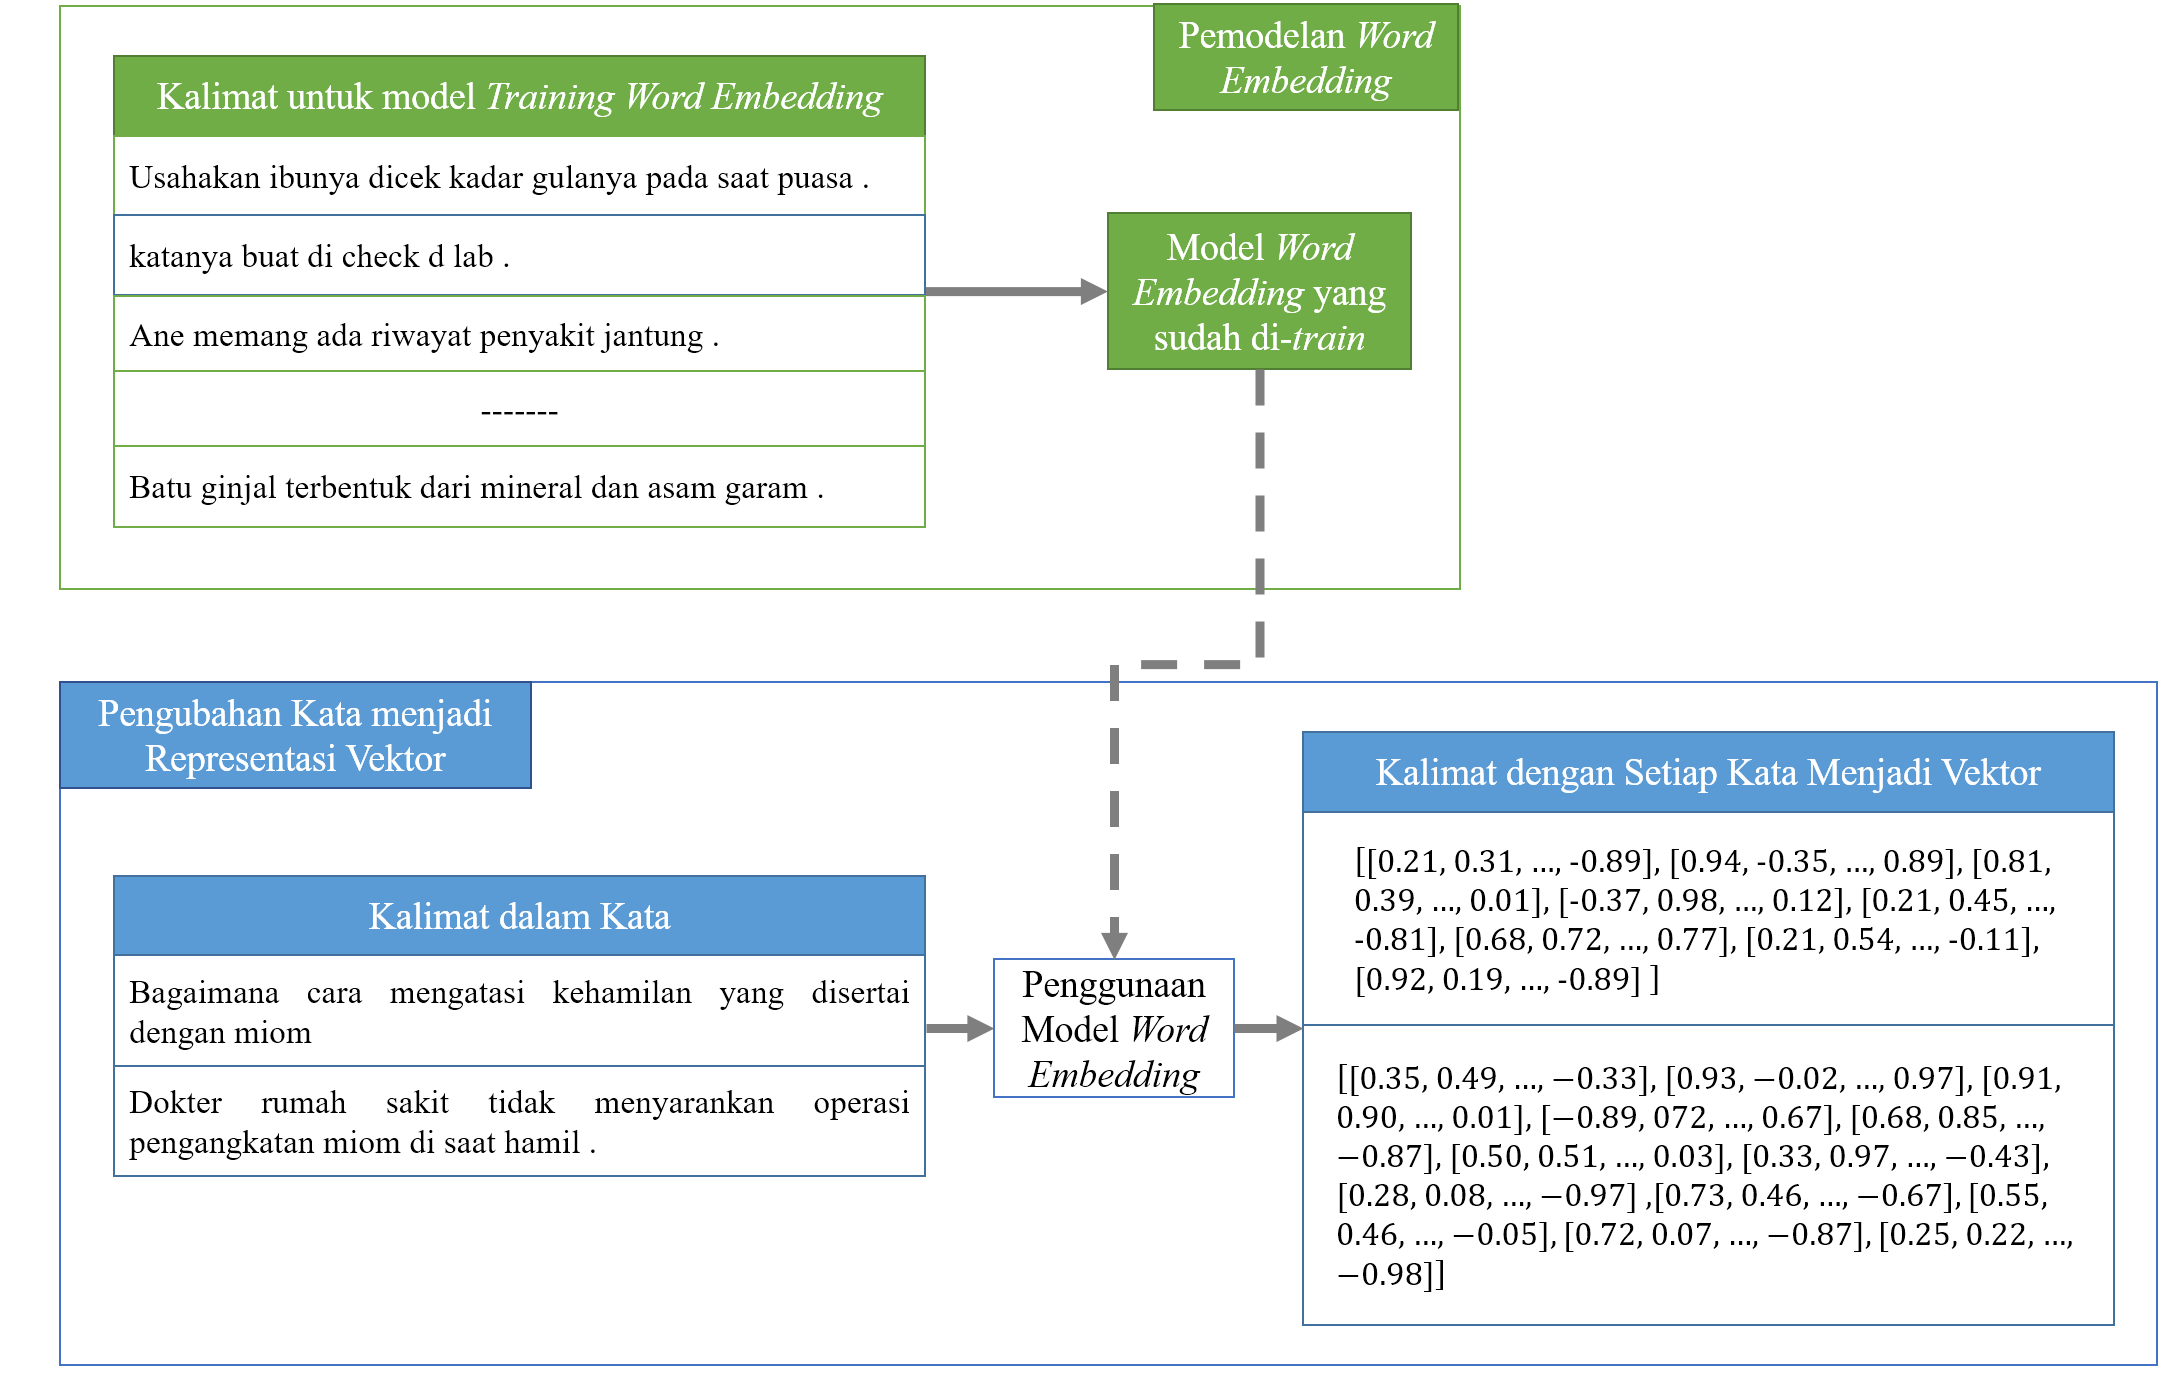
\includegraphics[width=\linewidth]{images/fiturkata}
	\caption{Ilustrasi Ekstraksi Fitur Kata pada Suatu Kalimat}
	\label{fig:fiturkata}
\end{figure}

\subsubsection{Part-of-Speech Tag (POS-Tag)}
POS Tag is a feature to represent the class of each word. In this research, we use POS Tag annotation which is mainly inspired by the work of Ruli Manurung (20XX). The POS Tags that we use are: Verb (V), Noun (NN), Adjective (ADJ), Adverb (ADV), Coordinative Conjunction (CC), Subordinative Conjunction (SC), Interjection (INTJ), Question (WH), Preposition (PREP), and Negation (NEG). Before feeding the feature to the deep learning model, we encode the POS tag features as a one-hot vector. Each one-hot vector represents each POS tag uniquely.

The example of POS Tag features is presented in Table~\ref{tab:examplepos}
\begin{table}
	\centering
	\caption{An example of POS Tag feature and its respective one-hot-vector}
	\label{tab:examplepos}
	\begin{tabular}{|lcccc|}
		\hline
		\textbf{Sentence} 				& Aku & pengen & makan & ayam \\
		\hline
		\textbf{POS Tag}				& NN & ADV & V & NN  \\
		\hline
		\textbf{One-Hot-Vector}		& [1, 0, 0, .., 0] & [0, 1, 0, .., 0] & [0, 0, 1, .., 0] & [0, .., 1, 0, 0] \\
		\hline
	\end{tabular}
\end{table}

While most of the deep learning research aims for not using such feature, we argue that POS tag is still important for building a robust model in our case. This is because of the fact that size of our corpus is relatively small compared to the huge English-based SRL corpus such as ConLL 2015 by~\cite{carreras2005introduction}. We argue that having Verb as one of our POS Tag will help to determine which one is the predicate, since predicate is usually in a form of verb, though some can also be adjectives. As the arguments having semantic role are mostly in a form of Noun, POS Tag Noun will be a helpful information as well. Other POS tags will help to determine which word that obviously does not have any semantic role.

In this work, we use gold-standard POS tag on our data as the features to prevent propagation errors from the POS tag model. This way, we can focus on analyzing errors resulting from the SRL model later in chapter 5. 

\subsubsection{Neighboring Word Embeddings}
Neighboring word embeddings are the vector representations of words located before and after the word being processed. We use specifically one word before and after the word being processed. Suppose that we are processing the word $w_{t}$ at time step $t$, the neighboring words embeddings are the vector representations of the word $w_{t-1}$ and $w_{t+1}$. We argue that this feature can be useful for capturing the context of the word by looking at the surrounding words. Suppose that the machine is processing the word \textit{"rumah"} in \textit{"aku tidur di rumah"}. By looking at the previous word, which is the preposition \textit{"di"}, it gives a hint that \textit{"rumah"} might have the semantic role \location.

\subsection{Model Architecture}
Recurrent Neural Networks (RNN) has a nature advantage for solving sequence labeling problem~\cite{zhou2015end}. ~\cite{hochreiter1997long} proposed Long Short-Term Memories (LSTM) as the specific version of RNN designed to overcome vanishing and exploding gradient problem. In this research, we experiment on various LSTM architectures, namely vanilla Long Short-Term Memories (LSTM), Bi-Directional LSTM (BLSTM), Convolutional Neural Network BLSTM (CNN-BLSTM), and Context-Aware BLSTM (CA-BLSTM). Each architecture is built incrementally upon the previous architectures, starting from the vanilla LSTM. The last architecture, CA-BLSTM, is the one we propose in this work.

\subsubsection{Vanilla LSTM}
% Explain what is LSTM (generally)
Vanilla LSTM is the basic, one-directional LSTM networks designed to overcome vanishing and exploding gradient problem found in RNN. To do so, it has forget gates, a gate to open or close incoming information from the previous time steps. We firstly explain the LSTM networks as the big picture for solving sequence labeling problem, followed by the details of every LSTM unit. 

% Gambar Big Picture LSTM
\begin{figure}
	\centering
	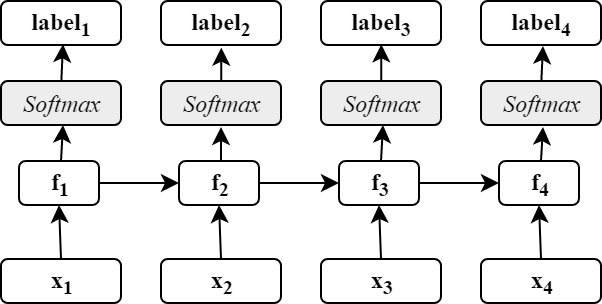
\includegraphics[width=0.75\linewidth]{images/olstm}
	\caption{An architecture of Context-Aware Bi-Directional Long Short Term Memories with total time step of 4}
	\label{fig:olstm}
\end{figure}

% Explain the formula based on big picture LSTM
Figure~\ref{fig:olstm} illustrates the big picture of the vanilla LSTM networks used in this research. Suppose that we have sequence of input tensors $[\mathbf{x_{1}}; \mathbf{x_{2}}; ...; \mathbf{x_{n}}]$, with $n$ denotes the number of time steps. Each input tensor $\mathbf{x_{t}}$ represents features of the word in time step $t$. For every time step $t$, each input tensor $\mathbf{x_{t}}$ is fed into the LSTM layer, resulting tensor $\mathbf{f_{t}}$, as shown in Equation~\ref{eq:lstm}. 

\begin{equation}
\label{eq:lstm}
\mathbf{f_{t}} = LSTM(\mathbf{x_{t}})
\end{equation}

Equation~\ref{eq:softmaxout} shows that each LSTM output from every time step is then processed by the time-distributed softmax layer to produce the probabilities of every possible label.

\begin{equation}
\label{eq:softmaxout}
label_{t} = Softmax(\mathbf{f_{t}})
\end{equation}

In each time step, label with highest probability among others will be the final output. This way, we have all the predicted labels for every time step.

After explaining the big picture of LSTM networks, we describe the details of every LSTM unit in time step $t$ shown in Equation~\ref{eq:lstm}. That is, given an input tensor $\mathbf{x_{t}}$, each LSTM unit will output tensor $\mathbf{f_{t}}$. Figure~\ref{fig:lstmunit} illustrates the architecture of one LSTM unit in time step $t$.

% Gambar single unit LSTM
\begin{figure}
	\centering
	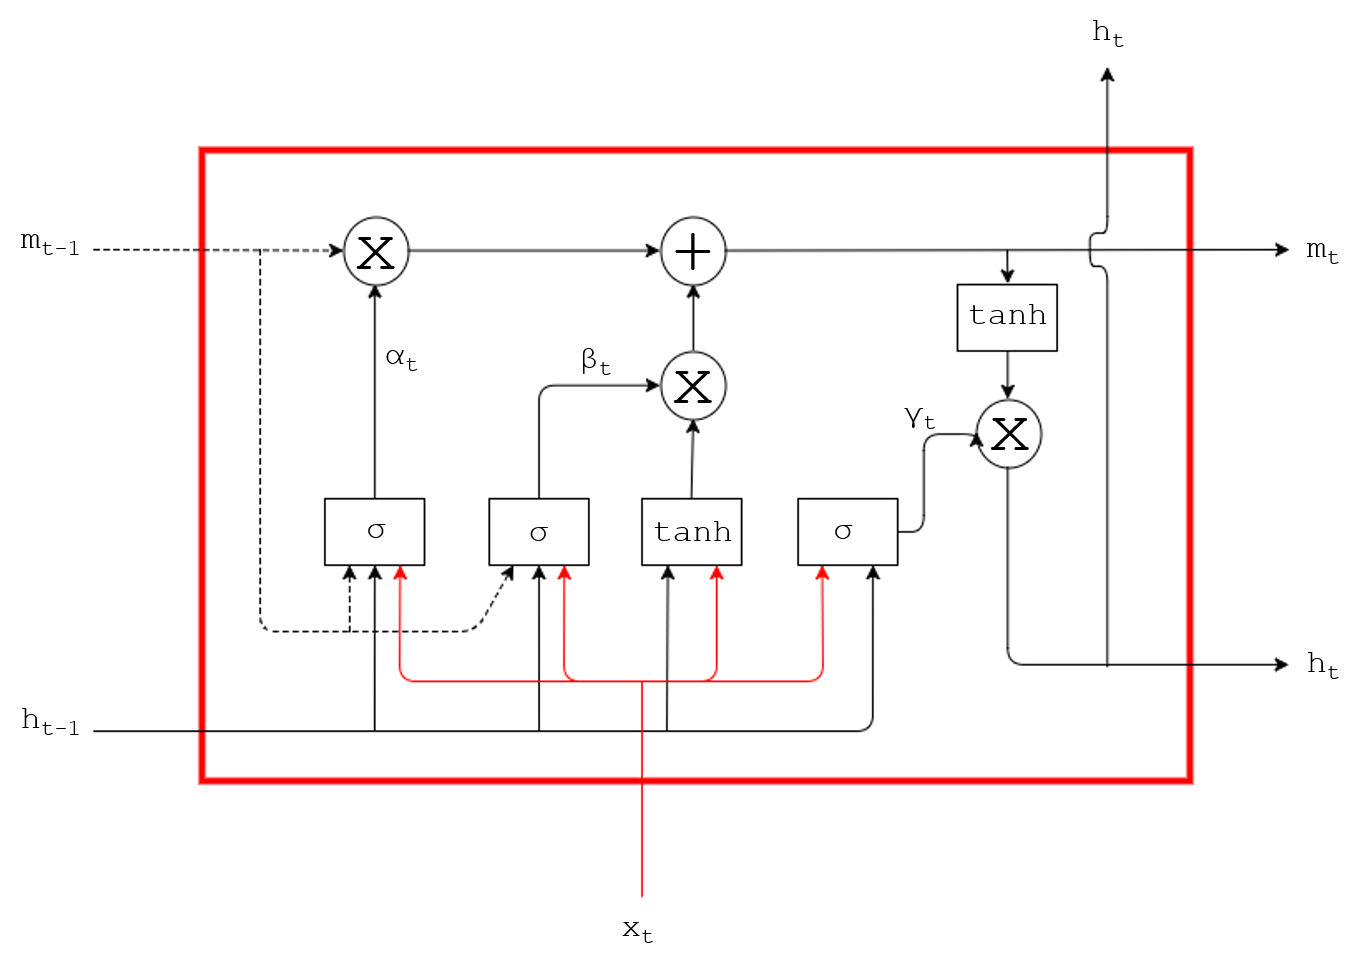
\includegraphics[width=0.85\linewidth]{images/lstm}
	\caption{An LSTM unit in time step $t$}
	\label{fig:lstmunit}
\end{figure}

% Explain the formula based on single cell LSTM
The LSTM unit in time step $t$ requires an input tensor $a_{t}$. As explained in subchapter X, the equations to produce output tensor $\mathbf{f_{t}}$ are presented as follows:

\begin{equation}\label{eq:lstmm}
m_{t}=\alpha_{t} (\times) m_{t-1} + \beta_{t} (\times) f(x_{t},{t-1})
\end{equation}
\begin{equation}\label{eq:lstmh}
h_{t}=\gamma_{t} (\times) tanh(m_{t})
\end{equation}
where
\begin{equation}\label{eq:lstmx}
f(x_{t},{t-1})=tanh(W_{xm} \cdot x_{t} + W_{hm} \cdot h_{t-1})
\end{equation}

$ \alpha_t $, $ \beta_t $, and $ \gamma_t $ are the gates:
\begin{enumerate}
	\item \textit{Forget gates}: $ \alpha_{t}=\sigma(W_{x\alpha} \cdot x_{t}+W_{h\alpha}\cdot~h_{t-1}+W_{m\alpha}\cdot~m_{t-1}) $
	\item \textit{Input gates}: $ \beta_{t}=\sigma(W_{x\beta}\cdot x_{t}+W_{h\beta}\cdot~h_{t-1}+W_{m\beta}\cdot~m_{t-1}) $
	\item \textit{Output gates}: $ \gamma_{t}=\sigma(W_{x\gamma}\cdot x_{t}+W_{h\gamma}\cdot~h_{t-1}+W_{m\gamma}\cdot~m_{t-1}) $
\end{enumerate}

It is worth noting that the LSTM layer is recursive, meaning that one of the inputs comes from the output of previous time step. This way, the result of each time step also depends on the previous ones.


\subsubsection{Bi-Directional LSTM (BLSTM)}
\label{sec:blstm}
% What is Bi-Directional LSTM generally, what it's for. Menurut Zhou gimana
Bi-Directional LSTM (BLSTM) is a modification of LSTM networks. While vanilla LSTM only goes one direction, BLSTM goes both ways in order to capture context information from the past and future, as explained by~\cite{zhou2015end}. This characteristic is suitable for SRL task, since information from the right (future) might be useful to determine the label of current time step, as explained by~\cite{zhou2015end}. The idea is to have two LSTM layers, one for going forward and another for going backward, as illustrated in Figure~\ref{fig:bilstm}

% Gambar BILSTM
\begin{figure}
	\centering
	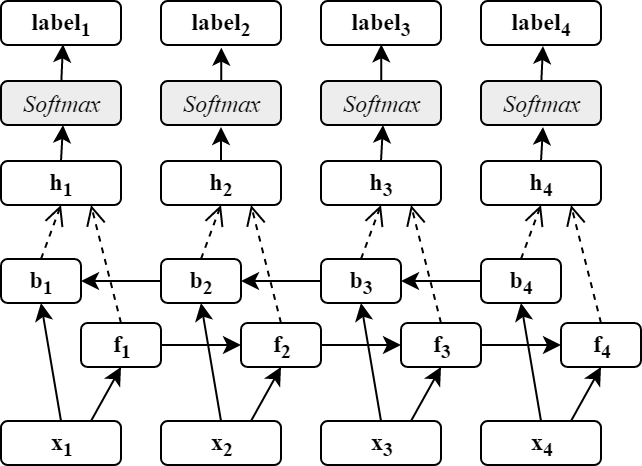
\includegraphics[width=0.75\linewidth]{images/blstm}
	\caption{An architecture of Context-Aware Bi-Directional Long Short Term Memories with total time step of 4}
	\label{fig:bilstm}
\end{figure}

% Explain the formula based on big picture BILSTM
Figure~\ref{fig:bilstm} shows that the input $\mathbf{x_{t}}$ in every time step $t$ is fed into two LSTM layers, the first one for going forward and the second one for going backward. These are illustrated in Equation~\ref{eq:lstmforward} and Equation~\ref{eq:lstmbackward}
\begin{equation}
\label{eq:lstmforward}
\mathbf{f_{t}} = ForwardLSTM(\mathbf{x_{t}})
\end{equation}

\begin{equation}
\label{eq:lstmbackward}
\mathbf{b_{t}} = BackwardLSTM(\mathbf{x_{t}})
\end{equation}

In each time step, the result tensors $mathbf{f_{t}}$ and $mathbf{b_{t}}$ are then concatenated to be one tensor output $\mathbf{h_{t}}$, as shown in Equation~\ref{eq:lstm_concat}
\begin{equation}
\label{eq:lstm_concat}
\mathbf{h_{t}} = Concatenate(\mathbf{f_{t}}, \mathbf{g_{t}})
\end{equation}

Likewise in vanilla LSTM architecture, the output tensor $\mathbf{h_{t}}$ is then fed into softmax layer, as shown in Equation~\ref{eq:bilstm_softmax}

\begin{equation}
\label{eq:bilstm_softmax}
label_{t} = Softmax(\mathbf{h_{t}})
\end{equation}

After which, the output of the softmax layer will determine the final label for each time step.

\subsubsection{CNN-BLSTM}
% What is CNN-BLSTM generally, what it's for.
In addition to the BLSTM architecture, we also experiment on adding Convolutional Neural Networks (CNN) layer underneath the BLSTM layer. The rationale is to capture raw context from the neighboring input tensors. This way, CNN can implicitly extract meaningful context information. Figure ~\ref{fig:cnnblstm} illustrates the big picture of the CNN-BLSTM architecture.

% Gambar CNN-BLSTM
\begin{figure}
	\centering
	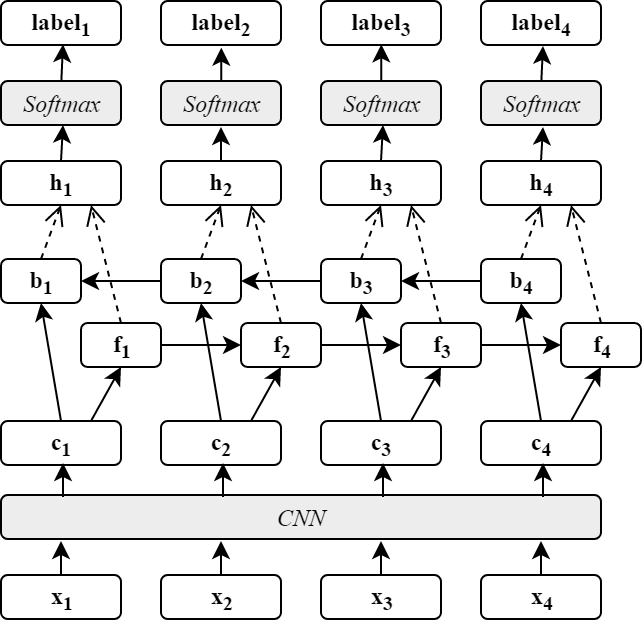
\includegraphics[width=0.75\linewidth]{images/cnnblstm}
	\caption{An architecture of Context-Aware Bi-Directional Long Short Term Memories with total time step of 4}
	\label{fig:cnnblstm}
\end{figure}

% Explain the formula based on big picture CNN-BILSTM
Instead of feeding the BLSTM with raw input tensor $\mathbf{x_{t}}$, CNN-BLSTM firstly processes it through CNN layer, resulting output tensor $\mathbf{c_{t}}$, as shown in Equation~\ref{eq:cnn}.
\begin{equation}
[\mathbf{c_{1}}; \mathbf{c_{2}}; ...; \mathbf{c_{n}}] = CNN([\mathbf{x_{1}}; \mathbf{x_{2}}; ...; \mathbf{x_{n}}])
\end{equation}

The result tensor $\mathbf{c_{t}}$ is then fed into the BLSTM layer, as explained in section~\ref{sec:blstm}. To simplify the notation, the BLSTM layer equation is summarized as follows.
\begin{equation}
\mathbf{h_{i}} = BLSTM(\mathbf{c_{i}})
\end{equation}

As explained in section~\ref{sec:blstm}, the BLSTM's output tensor $\mathbf{h_{i}}$ is then processed by the time-distributed softmax layer to determine the final output label.

\subsubsection{Context-Aware BLSTM (CA-BLSTM)}
% What is CA-BLSTM generally, what it's for
In this work, we propose a new LSTM architecture named Context-Aware Bi-Directional Long Short-Term Memory Networks (CA-BLSTM). The rationale is to add a dense yet useful high-level information containing a sentence context to every time step in order to help the machine to decide semantic roles better. With this in mind, we design an attention mechanism on top of the LSTM networks layers, as illustrated in Figure~\ref{fig:cabilstm} 

\begin{figure}
	\centering
	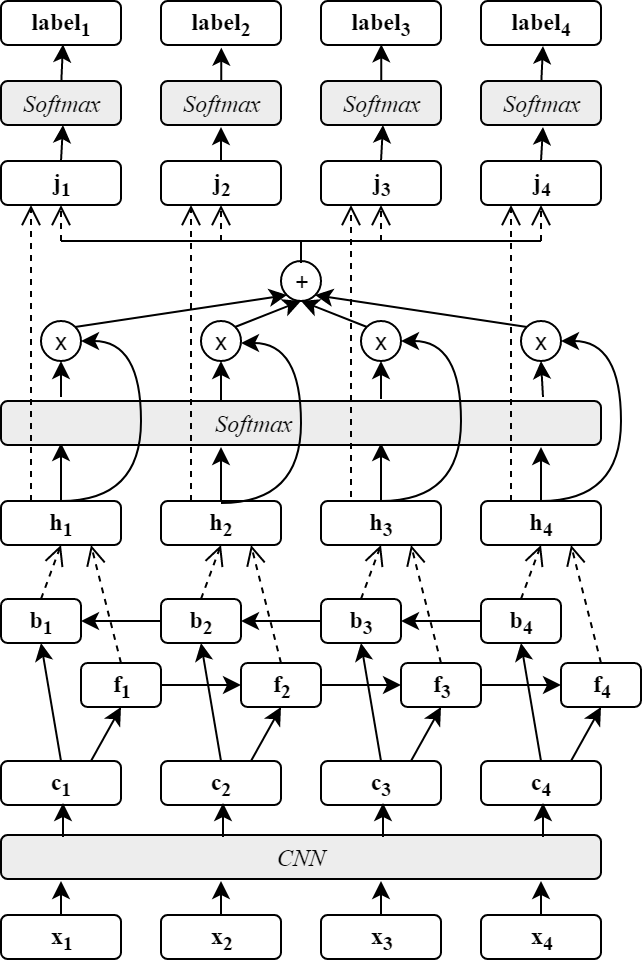
\includegraphics[width=0.75\linewidth]{images/cabilstm}
	\caption{An architecture of Context-Aware Bi-Directional Long Short Term Memories with total time step of 4}
	\label{fig:cabilstm}
\end{figure}

% Explain the formula based on big picture CA-BLSTM
The attention mechanism firstly collects the context information by multiplying trainable weights with all the vectors from every time step of the last LSTM output. We sum each element for each weighted vectors to reduce the dimension. The results are then fed into a hidden softmax layer which outputs weights with a total of 1. The original output vectors of the last LSTM output are multiplied by these distributed weights respectively. We then sum all the multiplication results as the final context information. The original LSTM outputs are concatenated with this context information before going to the last softmax layer to predict the semantic roles. 

We describe the formulation of the networks from the first layer all the way to the top. Like the previous architectures, it begins with these two equations:
\begin{equation}
[\mathbf{c_{1}}; \mathbf{c_{2}}; ...; \mathbf{c_{n}}] = CNN([\mathbf{x_{1}}; \mathbf{x_{2}}; ...; \mathbf{x_{n}}])
\end{equation}
\begin{equation}
\mathbf{h_{i}} = BLSTM(\mathbf{c_{i}})
\end{equation}

$\mathbf{x_{i}}$, $\mathbf{c_{i}}$, and $\mathbf{h_{i}}$ are the input tensors, the output of CNN layer, and the output of BLSTM layer respectively, with $i$ indicating the time step. 
\begin{equation}
\label{sum_weight}
g(\mathbf{h_{i}}) = Sum(\mathbf{W}.\mathbf{h_{i}})
\end{equation}

$\mathbf{h_{i}}$ is then fed into a differentiable neural networks function $g(\mathbf{h_{i}})$ in which it is multiplied by the time-distributed matrix $\textbf{W} \in {\rm I\!R^{H \times K}}$ and all the elements in it are summed. $H$ is the vector dimension of $\mathbf{h_{i}}$, meanwhile $K$ is the dimension size that we want as an output when we multiply \textbf{$W$} with $\mathbf{h_{i}}$.
\begin{equation}
[\alpha_{1}, \alpha_{2}, ..., \alpha_{n}] = Softmax([g(\mathbf{h_{1}}); g(\mathbf{h_{2}}); ..., g(\mathbf{h_{n}})])
\end{equation}
\begin{equation}
\mathbf{r_{i}} = \alpha_{i}.\mathbf{h_{i}}
\end{equation}

Once we have all the values of $[g(\mathbf{h_{1}}); g(\mathbf{h_{2}}); ...; g(\mathbf{h_{n}})]$, we make it as an input for the softmax layer, resulting weights $[\alpha_{1}; \alpha_{2}; ...; \alpha_{n}]$. All the original LSTM outputs $[\mathbf{h_{1}}; \mathbf{h_{2}}; ...; \mathbf{h_{n}}]$ are multiplied by these weights, with the results of $[\mathbf{r_{1}}; \mathbf{r_{2}}; ...; \mathbf{r_{n}}]$

\begin{equation}
\mathbf{z} = \mathbf{r_{1}} + \mathbf{r_{2}} + ... + \mathbf{r_{n}}
\end{equation}
\begin{equation}
\mathbf{j_{i}} = Concatenate(\mathbf{h_{i}}, z)
\end{equation}

We then sum all these vectors element-wise to have a context tensor $\mathbf{z}$. 
All the original LSTM outputs are thus concatenated with tensor $\mathbf{z}$ as the additional information to predict the semantic roles.
\begin{equation}
label_{i} = Softmax(\mathbf{j_{i}})
\end{equation}

Lastly, the time-distributed softmax layer produces the final semantic roles label.

\section{Experiment}
The annotated data is split into training, validation, and testing set with ration 60:20:20. We train our model by using training set. The trained model is then use to predict the semantic roles out of validation set. The analysis done in each experiment scenario is based on the result of our validation set. Lastly, the results of testing set will be used as the final metrics to compare between scenarios.

\section{Evaluation}
In each scenario, we evaluate the trained model in order to see how good it predicts the semantic roles as expected. The metrics for our evaluation are precision, recall, and F1. These metrics is applied to all semantic role labels. We then average each metrics from all semantic role labels to get the average precision, recall, and F1 of a model. The evaluation approach used is partial match in which a set of predicted labels is counted right if there is an intersection with the gold-standard \citep{seki2003probabilistic}. 

Suppose that we are evaluating the semantic role \patient. The rules for evaluation using partial match for semantic role \patient are explained as follows.

\begin{enumerate}
	\item Counting \textit{True Positive} (TP)\\
	For every gold standard label that has intersection with the predicted label, the value of True Positive ($TP$) is added by 1.
	\\
	
	\fbox{%
		\parbox{1.0\linewidth}{%
			Gold-standard: Aku pengen makan <Patient>\textbf{ayam goreng}</Patient> deh\\
			Predicted.1: Aku pengen makan <Patient>\textbf{ayam goreng}</Patient> deh\\
			Predicted.2: Aku pengen makan <Patient>\textbf{ayam}</Patient> goreng deh\\
			Predicted.3: Aku pengen makan <Patient>\textbf{ayam goreng deh} </Patient>\\
			Predicted.4: Aku pengen makan ayam goreng deh
		}%
	}
	\\
	
	The examples above illustrate four scenarios of possible predicted results, denoted as Predicted.1, Predicted.2, Predicted.3, and Predicted.4, given a gold-standard called Expected which has "ayam goreng" as the \patient.
	\\
	
	Predicted.1 predicts exactly the same as the Expected, hence the value of $TP$ is added by 1. The result of Predicted.2 has an intersection with the gold-standard, which is "ayam", the value of $TP$ is then added by 1 as well. Although Predicted.3 predicts too much as it includes "deh" as part of \patient, it also has an intersection with the gold-standard, which is "ayam goreng". The Predicted.3 therefore also adds the value of $TP$ by 1. Meanwhile, Predicted.4 does not predict anything. In this case, the value of $TP$ is not added at all.
	\\
	
	\item Counting \textit{False Positive} (FP)\\
	For every predicted label that should not be predicted according to gold-standard, the value of False Positive ($FP$) is added by 1.
	\\
	
	\fbox{%
		\parbox{1.0\linewidth}{%
			Gold-standard: Aku pengen makan <Patient>\textbf{ayam goreng}</Patient> deh\\
			Predicted.1: <Patient>Aku</Patient> pengen makan ayam goreng deh\\
		}%
	}
	\\
	
	From the example above, "Aku" is predicted as \patient, while it should not be predicted as \patient according to the gold-standard. This will add the value of $FP$ by 1.
	\\
	
	\item Counting \textit{False Negative} (FN)\\
	For every gold-standard label that is either not predicted or predicted with wrong label, the value of False Negative ($FN$) is added by 1.
	\\
	
	\fbox{%
		\parbox{1.0\linewidth}{%
			Gold-standard: Aku pengen makan <Patient>\textbf{ayam goreng}</Patient> deh\\
			Predicted.1: Aku pengen makan <Agent>\textbf{ayam goreng}</Agent> deh\\
			Predicted.2: Aku pengen makan ayam goreng deh
		}%
	}
	\\
	
	From the example above, Predicted.1 predicts "ayam goreng" as \agent, while it should be predicted as \patient. In this case, the value of $FP$ is added by 1. Predicted.2 illustrates an example which does not predict "ayam goreng" with any label, while it should be predicted as \patient. In this case, the value of $FP$ is added by 1 as well.
	
\end{enumerate}

After we have the value of $TP$, $FP$, and $FN$ for the semantic role \patient, we then count the precision, recall, and F1 with following equations:
\begin{align}
Precision &= \frac{TP}{TP+FP}\\
Recall &= \frac{TP}{TP+FN}\\
F-Measeure &= 2 \cdot \frac{Precission \cdot Recall}{Precission + Recall}
\end{align}

Other semantic roles, such as \agent and \beneficiary, are also evaluated by following these rules. After we have the value of precision, recall, and F1 for every semantic role, we average them to get the average precision, recall, and F1 for the model being evaluated.
	